\chapter{T2K and SK Experiment Overview}
\label{chap:T2KSKExp}

\finish{This needs some references!}

\section{The Super-Kamiokande Experiment}
\label{sec:T2KSKExp_SK}

The SK experiment began taking data in 1996 and has had many modifications throughout its lifespan. There has been six defined periods of data taking as noted in \autoref{tab:T2KSKExp_SKPeriods}. Between the SK-I and SK-II periods, a significant proportion of the PMTs were damaged during maintainence. Those that survived were equally distributed throughout the detector in the SK-II era, which resulted in a reduced photo-coverage. From SK-III onwards, significant repair efforts were made such that the full suite of PMTs were operational. Before the start of SK-IV, the data acquisition and electronic systems were upgraded. Between SK-IV and SK-V, a significant effort was placed into tank open maintainence and repair/replacement of defective PMTs, a task in which the author of this thesis was required for. Consequently, the detector conditions were significantly different between the two operational periods. SK-VI saw the start of the \quickmath{0.01\%} gadonlium doped water being introduced into the tank and the detector continues to operate to this day. Efforts are currently underway to increase the gadolinium concentrate in the likely start of the next SK period.

\begin{table}[ht!]
    \centering
    \begin{tabular}{c|l|l|c}
      \hline
      Period & Start Date & End Date & Live-time (days) \\
      \hline
      I & April 1996 & July 2001 & 1489.19 \\
      II & October 2002 & October 2005 & 798.59 \\
      III & July 2006 & September 2008 & 518.08 \\
      IV & September 2008 & May 2018 & 3244.4 \\
      V & January 2019 & July 2020 & 461.02 \\
      VI & July 2020 & Ongoing & 583.3 \\
      \hline 
      \hline
    \end{tabular}
    \caption{The various SK periods and respective live-time. The SK-VI live-time is calculated until \quickmath{1^{\text{st}}} April 2022.}
    \label{tab:T2KSKExp_SKPeriods}
\end{table}

\subsection{The SK Detector}
\label{subsec:T2KSKExp_SKDetector}

The basic structure of the Super-Kamiokande (SK) detector is a cylindrical tank with diameter \quickmath{39.3\text{m}} and hieght \quickmath{41.1\text{m}} filled with ultrapure water. A diagram of the signficant parts of the SK detector is illustrated in \autoref{fig:T2KSKExp_SK_Diag}. The SK detector is situated in the Kamioka mine in Gifu, Japan. The cavern in which the detector is located is underground with roughly \quickmath{1\text{km}} rock overburden (\quickmath{2.7 \text{km}} water equivalent overburden). At this depth, the rate of cosmic ray muons is significantly decreased to a value of \quickmath{\approx 2\text{Hz}}, compared to a surface-level detector. The top of the tank is covered with stainless steel which is designed as a working platform for maintainence, calibration and location for high voltage and data acquisition electronics.

\begin{figure}[h]
  \begin{subfigure}[t]{0.95\textwidth}
    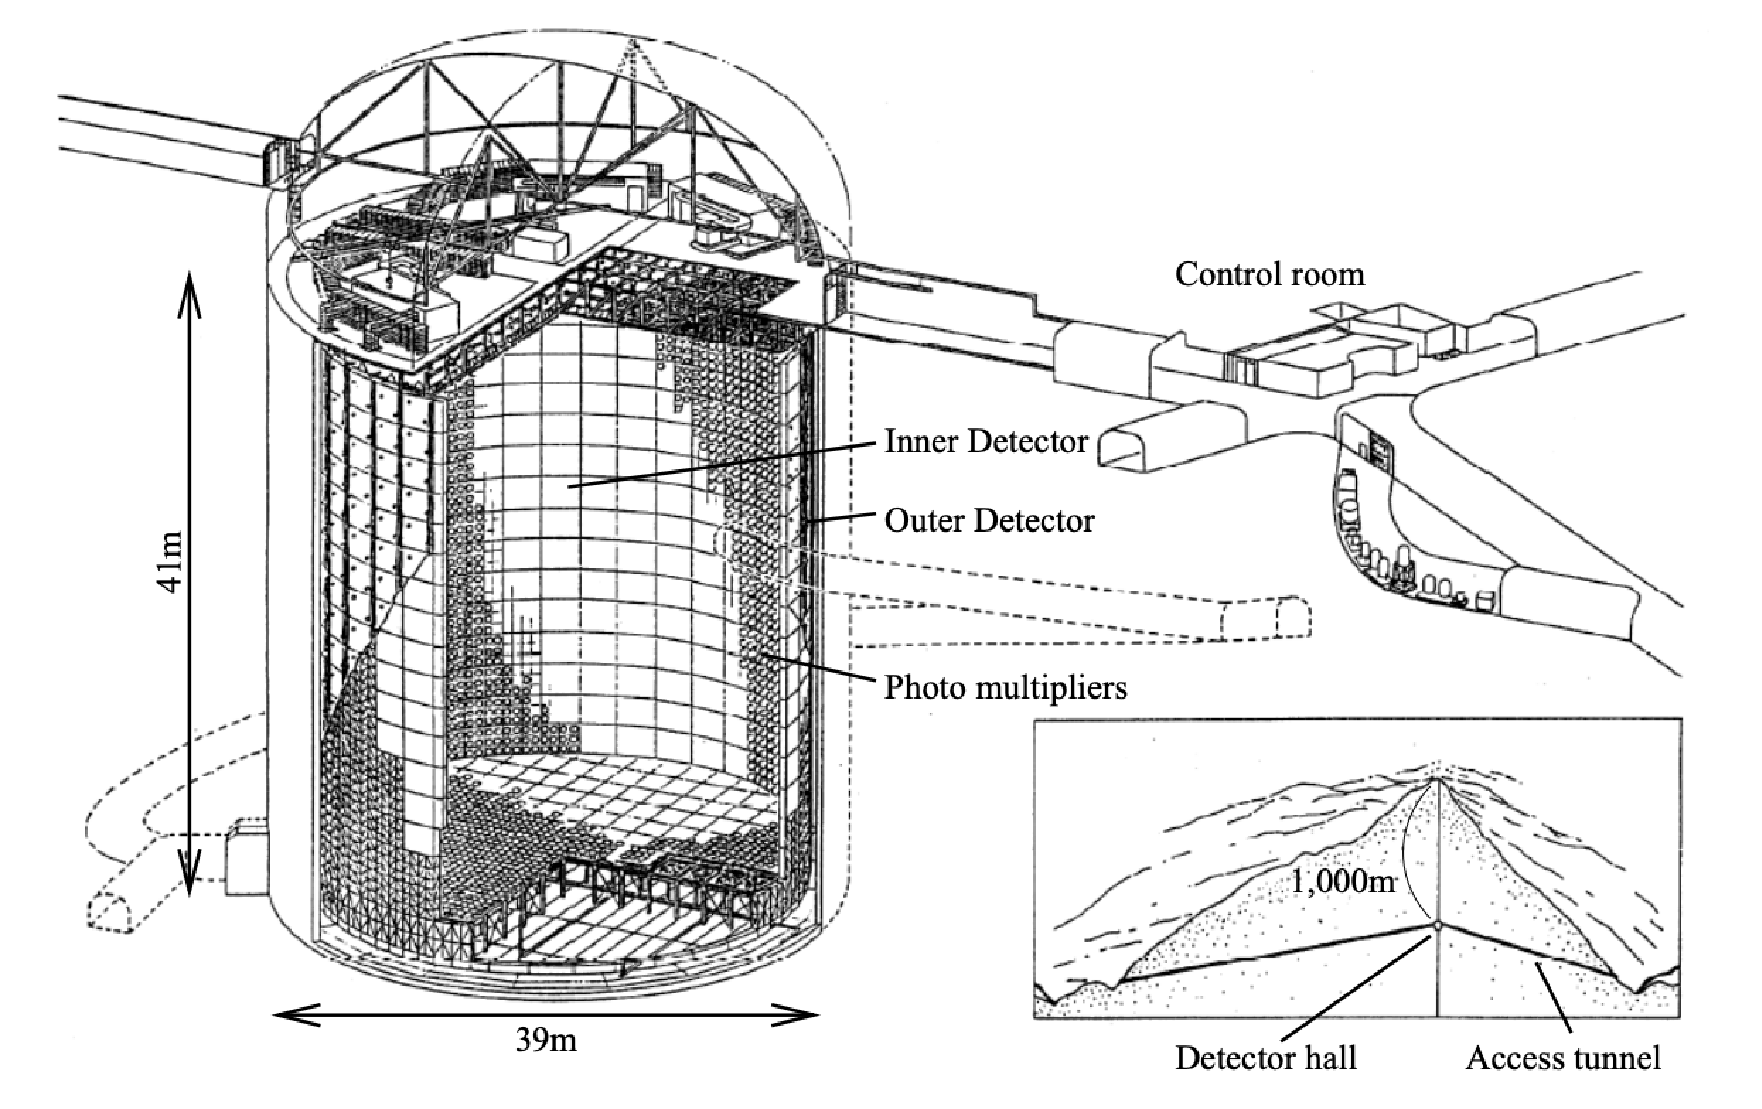
\includegraphics[width=\textwidth, trim={0mm 0mm 0mm 0mm}, clip,page=1]{Figures/Detectors/SKDiagram.pdf}
  \end{subfigure}
  \caption{A schematic diagram of the Super-Kamiokande Detector. Taken from \cite{Itow2001-bc}.}
  \label{fig:T2KSKExp_SK_Diag}
\end{figure}

A smaller cylindrical structure (\quickmath{36.2\text{m}} diameter, \quickmath{33.8\text{m}} hieght) is situated inside the tank, with an approximate \quickmath{2\text{m}} gap between this structure and the outer tank wall. The purpose of this structure is to support the photomultiplier tubes (PMTs). The volume inside and outside the support structure are referred to as the inner detector (ID) and outer detector (OD), respectively. The ID and OD are instrumented by \quickmath{11129} \quickmath{50\text{cm}} and \quickmath{1885} \quickmath{20 \text{cm}} PMTs respectively. The inner detector contains a \quickmath{32\text{kton}} volume of water, although many analyses performed at SK use a ``fiducial volume'' defined by the volume of water inside the ID excluding some distance to the ID wall. This reduces the volume of detector which is sensitive to neutrino events but reduces radioactive backgrounds and allows for better constraints on the reconstruction systematics. The nominal fiducial volume is defined as the area contained inside \quickmath{2\text{m}} from the ID wall for a total of \quickmath{22.5\text{kton}} water.

The two regions of the detector (ID and OD) are optically separated with opaque black plastic. The purpose of this is to deteremine whether a track entered or exited the ID. This allows cosmic muon rays and partially contained events to be tagged and separated from neutrino events entirely contained within the detector's sensitive region. This black plastic is also used to cover the area between the ID PMTs to reduce photon reflection from the ID walls. Contrary to this, the OD is lined with a reflective material (called Tyvek) to allow photons to reflect around inside the OD until collected by one of the PMTs. Furthermore, each OD PMT is backed with \quickmath{50\times50\text{cm}} plates of wavelength shifting acrylic which increases the efficiency of light collection.

In the SK-IV data taking period, the photocathode coverage of the detector, or the fraction of the ID wall instrumented with PMTs, is \quickmath{\sim 40\%}. The PMTs have a quantum efficiency (the ratio of detected electrons to incident photons) of \quickmath{\sim 21\%}. The proportion of photoelectrons which produce a signal in the dynode of a PMT, termed the collection efficiency, is \quickmath{>70 \%}. One disadvantage of using PMTs as the detection media is that the Earth's geomagnetic field can modify their response. Therefore, a set of compensation coils is built around the inner surface of the detector to mitigate this effect.

As mentioned, the SK detector is filled with ultrapure water, which in a perfect world would contain no impurities. However bacteria and organic compounds can significantly degrade the water quality, thus decreasing the attenuation length thus reducing the total number of photons which could be detected by the PMTs. To combat this, a sophisticated water treatment system has been developed for SK. UV lights, mechanical filters and membrane degasifiers are used to reduce the bacteria, suspended particulates and radioactive materials from the water. The flow of water within the tank is also critical as it can remove stagnant bacterial growth or build up of dust on the surfaces within the tank. Gravity drifts impurities in the water towards the bottom of the tank which if left uncontrolled, can create assymetric water conditions between the top and bottom of the tank.
%The flow of water in the tank can be controlled via mechanically driven circulation or temperature driven convection.
Typically, the water entering the tank is cooled below the ambient temperature of the tank to control convection and inhibit bacteria growth. Furthermore, the dark noise hits within PMTs is sensitive to the PMT temperature so controlling the temperature gradients within the tank is beneficial for stable measurements.

SK-VI is the first phase of the SK experiment to use gadonlium dopants within the ultrapure water. As such, the SK water system had to be replaced to avoid removing the gadolium concentrate from the ultrapure water. For an inverse \quickmath{\beta}-decay (IBD) interaction in a water target, the emitted neutron is thermally captured on hydrogen. This process releases \quickmath{2.2 \text{MeV}} \quickmath{\gamma} rays which are difficult to detect due to Compton scattered elecrtons from a \quickmath{\gamma} ray of this energy is very close to the Cherenkov threshold, limiting the number of photons produced. Thermal capture of neutrons on gadolinium generates \quickmath{\gamma} rays with higher energy meaning they are more easily detected. SK-VI has \quickmath{0.01 \%} Gd loading (\quickmath{0.02\%} gadolinium sulphate by mass) which causes \quickmath{\approx 50\%} of neutrons emitted by IBD to be captured on gadolinium. Whilst predominantly useful for low energy analyses, Gd loading allows \quickmath{\nu/\bar{\nu}} separation for atmopsheric neutrino event selections \cite{Marti2019-gu}. Efforts are currently in place to increase the gadolinium concentrate to \quickmath{0.03 \%} for \quickmath{\approx 75\%} neutron capture efficiency on gadonlium. The final stage of loading targets \quickmath{0.1 \%} concentrate.

\subsection{Triggering and Calibration}
\label{subsec:T2KSKExp_SKTriggeringCalib}

The calibration of the SK detector is documented in \cite{Abe_2014_SKCalib} and summarised below.

Before installation, \quickmath{420} PMTs were calibrated to have identical charge response and then distributed throughout the tank in a cross-shape pattern (As illustrated by \autoref{fig:T2KSKExp_SK_StandardPMTs}). These are used as a standardised measure for the rest of the PMTs installed at similar geometric positions within SK to be calibrated against. This allows each PMT to have it's high voltage set so that all PMTs give the same signal for an identical light collection. To perform this calibration, a xenon lamp is located at the center of the SK tank which flashes uniform light at \quickmath{1 \text{Hz}}. This allows for geometrical effects, water quality variation and timing effects to be measured in-situ throughout normal data taking periods.

\begin{figure}[h]
  \begin{subfigure}[t]{0.50\textwidth}
    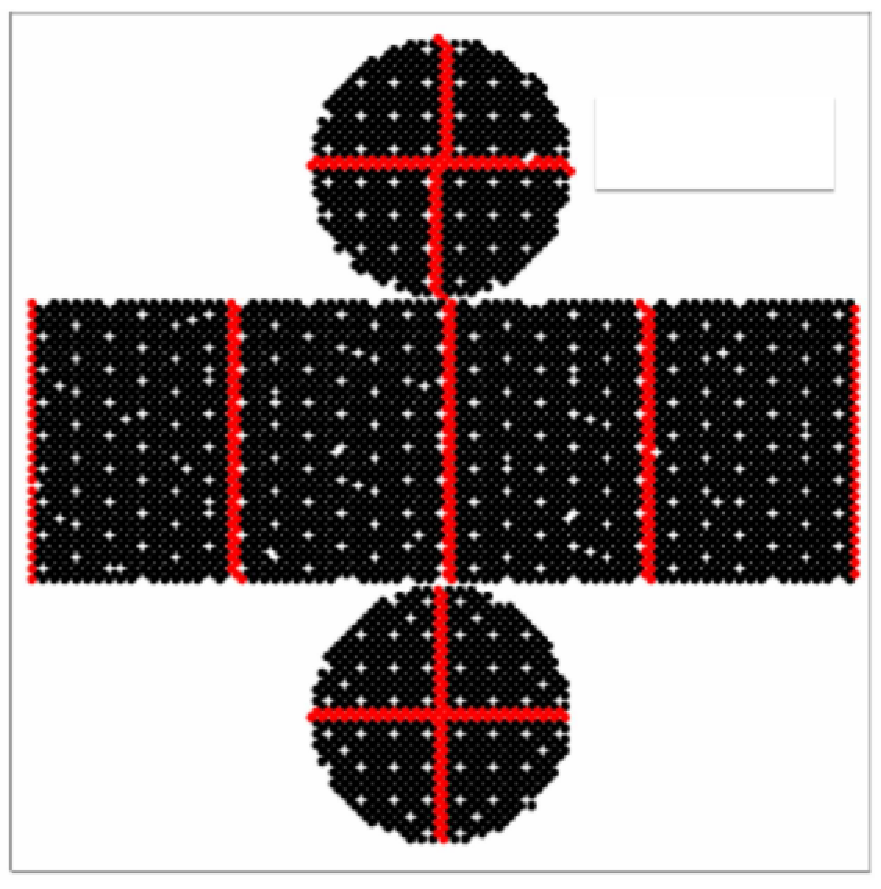
\includegraphics[width=\textwidth, trim={0mm 0mm 0mm 0mm}, clip,page=1]{Figures/Detectors/StandardPMTs.pdf}
  \end{subfigure}
  \caption{The location of ``standard PMTs'' (red) inside the SK detector. Taken from \cite{Abe_2014_SKCalib}.}
  \label{fig:T2KSKExp_SK_StandardPMTs}
\end{figure}

The ``gain'' of a PMT is defined as the ratio of total charge of the signal produced compared to the charge of photoelectrons emitted by the photocathodes within the PMT. To calibrate the signal of each PMT, the ``relative'' and ``absolute'' gain values are measured. The relative gain is the variation of gain among each of the PMTs whereas the absolute gain is the average gain of all PMTs. 

The relative gain is calibrated as follows. A laser light is used to generate measurements under two conditions; a high-intensity flash which illuminates every PMT with a sufficient number of photons, and a low-intensity flash in which only a small number of PMTs collect light. The first measurement creates an average charge, \quickmath{Q_{obs}(i)} on PMT \quickmath{i}, whereas the second measurement ensures that each hit PMT only generates a single photoelectron. For the low intensity measurement, the number of times each PMT records a charge larger than some threshold value, \quickmath{N_{obs}(i)} is counted. \cite{Abe_2014_SKCalib} indicates that the specified threshold value does not induce any significant biases in the measurement of gain. The values measured can be expressed as,

\begin{equation}
  \begin{split}
    Q_{obs}(i) &\propto I_{H} \times f(i) \times \epsilon(i) \times G(i), \\
    N_{obs}(i) &\propto I_{L} \times f(i) \times \epsilon(i),
  \end{split}
\end{equation}

Where \quickmath{I_{H}} and \quickmath{I_{L}} is the intensity of the high and low flashes, \quickmath{f(i)} is the acceptance efficiency of the \quickmath{i^{\text{th}}} PMT, \quickmath{\epsilon(i)} is the product of the quantum and collection efficiency of the \quickmath{i^{\text{th}}} PMT and \quickmath{G(i)} is the gain of the \quickmath{i^{\text{th}}}	PMT. The relative gain for each PMT can determined by taking the ratio of these quantities.

The absolute gain calibration is performed by observing fixed energy \quickmath{\gamma}-rays of \quickmath{E_{\gamma} \approx 9\text{MeV}} emitted isotropically from neutron capture on a NiCf source situated at the centre of the detector. This generates a photon yeild of about \quickmath{0.004} photoelectrons/PMT/event, meaning that \quickmath{>99\%} of PMT signals are generated from a single photoelectron. A charge distribution is generated by performing this calibration over all PMTs, and the average value of this distribution is taken to be the absolute gain value. It has been found that the absolute gain increases as a function of time despite there being no known reason for this behaviour.

\finish{Include triggering}

\subsection{Cherenkov Radiation}
\label{subsec:T2KSKExp_Cherenkov}

Cherenkov light is emitted from any highly energetic charged particle travelling with relativistic velocity \quickmath{\beta} greater than the local speed of light in a medium with refractive index \quickmath{n>1.0}. This occurs due to the charged particle exciting the polarised media, which de-excites via photon emission. From Huygen's principal, the emitted waves propagate outwards but only generate coherent wavefronts when the charged particle moves faster than the phase velocity of that media. Consequently, Cherenkov light is formed at the surface of a cone with characteristic pitch angle,

\begin{equation}
  \label{eq:T2KSKExp_CherenkovConeAngle}
  \cos(\theta)=\frac{1}{\beta n}.
\end{equation}

Consequently, the Cherenkov momentum threshold (where the requirement is \quickmath{\beta = 1/n}) is dependent upon the mass, \quickmath{m}, of the charged particle moving through the media,

\begin{equation}
  P_{thres} = \frac{m}{\sqrt{n^{2}-1}}
\end{equation}

For water, where \quickmath{n = 1.33}, the Cherenkov threshold momentum and energy for various particles is given in \autoref{tab:T2KSKExp_CherenkovThreshold}. For completeness, \quickmath{\gamma}-rays are directed indirectly via the combination of photons generated by compton scattering and pair production. The threshold for detection in the SK detector is higher than the threshold for photon production. This is due to the fact that the attenuation of photons in the water means that typically \quickmath{\sim 75\%} of Cherenkov photons reach the ID PMTs. Then the collection and quantum efficiencies described in \autoref{subsec:T2KSKExp_SKDetector} results in the number of detected photons being lower than the number of photons which reach the PMTs. 

\begin{table}[ht!]
    \centering
    \begin{tabular}{l|c|c}
      \hline
      Particle & Threshold Momentum (MeV) & Threshold Energy (MeV)\\
      \hline
      Electron & 0.5828 & 0.7751 \\
      Muon & 120.5 & 160.3 \\
      Pion & 159.2 & 211.7 \\
      Proton & 1070.0 & 1423.1 \\
      \hline
      \hline
    \end{tabular}
    \caption{The threshold momentum and energy for a particle to generate Cherenkov light in ultrapure water, as calculated in \autoref{eq:T2KSKExp_CherenkovConeAngle} in ultrapure water where \quickmath{n = 1.33}.}
    \label{tab:T2KSKExp_CherenkovThreshold}
\end{table}

\finish{Plot of muon momentum showing difference between Cherenkov threshold and detected threshold}

\section{The Tokai to Kamiokande Experiment}
\label{sec:T2KSKExp_T2K}

\subsection{The Neutrino Beam}
\label{subsec:T2KSKExp_T2K_NeutrinoBeam}

\subsection{The Near Detector at \quickmath{280\text{m}}}
\label{subsec:T2KSKExp_T2K_ND280}

\subsection{The Interactive Neutrino GRID}
\label{subsec:T2KSKExp_T2K_INGRID}

